\documentclass[12pt]{article}

\setlength{\parindent}{0pt}
\setlength{\parskip}{0.30em}

\usepackage[utf8]{inputenc}
\usepackage[T1]{fontenc}
\usepackage[margin=1in]{geometry}
\usepackage{amsmath, amssymb}
\usepackage{booktabs}
\usepackage[font=small,labelfont=bf]{caption}
\usepackage{enumitem}
\usepackage{etoolbox}
\usepackage{float}
\usepackage{graphicx}
\usepackage{hyperref}
\usepackage{setspace}

\setstretch{1.05}
\setlist{noitemsep, topsep=1pt, partopsep=0pt, parsep=0pt}
\setlength{\textfloatsep}{8pt plus 1pt minus 2pt}
\setlength{\floatsep}{8pt plus 1pt minus 2pt}
\setlength{\intextsep}{8pt plus 1pt minus 2pt}
\renewcommand{\arraystretch}{0.92}
\AtBeginEnvironment{tabular}{\small}
\newcommand{\best}[1]{\textbf{#1}}
\graphicspath{{../}{./}}
\hypersetup{
    colorlinks=true,
    linkcolor=black,
    citecolor=black,
    urlcolor=blue
}

\title{Comparative Classification Models for Loan Default Risk Prediction}
\author{Junfeng Nie}
\date{}

\begin{document}

\maketitle

\section{Motivation}

\subsection{Background}

Loan default prediction is a binary classification problem in credit-risk analysis. In this project, the response variable is \texttt{default}, where \texttt{default}=1 represents a defaulted loan and \texttt{default}=0 represents a non-defaulted loan. The predictors are applicant income, loan amount, and employment status.

The dataset is the \textit{Loan Default Prediction Dataset} published on Kaggle by Şahide Şeker \cite{seker_kaggle}. It is a synthetic dataset with 1000 observations and the columns \texttt{loan\_id}, \texttt{income}, \texttt{loan\_amount}, \texttt{employment\_status}, and \texttt{default}.

\subsection{Why the Problem Is Important}

Credit-risk decisions involve a direct tradeoff between risk control and access to credit. If a lender underestimates default risk, it may approve loans that are unlikely to be repaid. If it overestimates default risk, it may reject applicants who could have repaid successfully. A useful classification model should therefore do more than report a high overall accuracy. It should help identify high-risk borrowers while also making clear which features drive the prediction.

This project focuses on three pain points that commonly appear in credit-risk modeling:

\begin{enumerate}[label=(\roman*)]
    \item \textbf{Interpretability:} A lender may need to explain why the model assigns higher risk to one applicant than another. Logistic Regression is useful because its coefficients can be interpreted through log-odds and odds ratios.
    \item \textbf{Overlapping feature space:} Applicants with different default outcomes may have similar income and loan amount values. This overlap can make a single linear decision boundary insufficient.
    \item \textbf{Model complexity:} More flexible models may capture nonlinear structure, but they may also overfit. Polynomial expansion and regularization provide a controlled way to study this tradeoff.
\end{enumerate}

\subsection{Real-World Application}

In a real lending workflow, a model like this could support early credit-risk screening by estimating default risk from borrower characteristics. It would not replace full underwriting, but it captures the core task of identifying risky applications from structured financial data.

This project also serves as a methodological case study. Logistic Regression, kNN, and regularized polynomial Logistic Regression allow the same dataset to be studied from linear, local-distance, and nonlinear feature-expansion perspectives.

\section{Research Questions}

The analysis is organized around three research problems. Each problem is divided into concrete sub-problems so the analysis can connect model behavior, predictive performance, and feature effects.

\subsection{Linear Baseline and Feature Interpretation}

\textbf{Main question:} Can a linear probabilistic classifier provide a useful and interpretable baseline for predicting loan default from income, loan amount, and employment status?

\begin{enumerate}[label=\textbf{1(\alph*)}]
    \item Perform EDA and preprocessing: remove \texttt{loan\_id}, encode \texttt{employment\_status}, standardize continuous variables, and create a stratified train/validation/test split.
    \item Train a Logistic Regression baseline and evaluate it using test-set classification metrics and a confusion matrix.
    \item Interpret the learned coefficients, especially how unemployment changes default risk relative to the employed baseline group.
\end{enumerate}

\subsection{Local Geometry and k-Nearest Neighbors Classification}

\textbf{Main question:} Can a local distance-based classifier capture borrower-risk structure that the global linear Logistic Regression model cannot represent?

\begin{enumerate}[label=\textbf{2(\alph*)}]
    \item Implement kNN and test how standardized versus unstandardized features affect distance-based classification.
    \item Tune $k$ on the validation set and use the train/validation curve to discuss high variance and high bias.
    \item Compare the best kNN model with the Logistic Regression baseline on the same test metrics.
\end{enumerate}

\subsection{Polynomial Feature Expansion and Regularized Logistic Classification}

\textbf{Main question:} Can polynomial feature expansion improve Logistic Regression by representing nonlinear relationships, and can regularization control the additional complexity?

\begin{enumerate}[label=\textbf{3(\alph*)}]
    \item Expand \texttt{income} and \texttt{loan\_amount} into second-order polynomial and interaction features, then report the new feature dimension.
    \item Train L2- and L1-regularized Logistic Regression models and tune regularization strength on the validation set.
    \item Compare coefficient patterns and determine whether L1 produces sparse high-order or interaction terms.
\end{enumerate}

\section{Hypotheses}

\begin{enumerate}[label=(\roman*)]
    \item \textbf{Employment status and baseline risk:} the unemployed indicator is expected to increase predicted default risk, making employment status one of the strongest baseline predictors.
    \item \textbf{kNN and feature scaling:} kNN is expected to perform better after standardizing \texttt{income} and \texttt{loan\_amount}; very small $k$ should show high variance, while very large $k$ should show higher bias.
    \item \textbf{Polynomial expansion:} polynomial expansion is expected to improve Logistic Regression moderately if nonlinear income--loan amount relationships are present.
    \item \textbf{L1 and L2 regularization:} L1 regularization is expected to produce sparser coefficients than L2 by setting some high-order or interaction terms to zero.
\end{enumerate}

\section{Evaluation Criteria}

\subsection{Evaluation Metrics}

The project will be considered successful if all models are evaluated consistently using accuracy, precision, recall, $F_1$-score, and confusion matrices. For true positives (TP), true negatives (TN), false positives (FP), and false negatives (FN), the evaluation metrics are defined as
\[
\begin{aligned}
\text{Accuracy} \quad &=\quad \frac{TP + TN}{TP + TN + FP + FN}, \\
\text{Precision} \quad &=\quad \frac{TP}{TP + FP}, \\
\text{Recall} \quad &=\quad \frac{TP}{TP + FN}, \\
F_1 \quad &=\quad
\frac{2 \cdot \text{Precision} \cdot \text{Recall}}
{\text{Precision} + \text{Recall}}.
\end{aligned}
\]
Confusion matrices will be used to interpret the types of errors made by each model. Since this is a comparative modeling project rather than a deployment system, success is defined by internally consistent evaluation and interpretable comparison rather than by a fixed industrial performance threshold. A model is considered practically better only if it improves $F_1$-score while preserving reasonable precision and recall.

In the implementation, these quantities are computed with \texttt{sklearn.metrics} functions such as \texttt{accuracy\_score}, \texttt{precision\_score}, \texttt{recall\_score}, \texttt{f1\_score}, and \texttt{confusion\_matrix}. The confusion matrix reports the counts of true negatives, false positives, false negatives, and true positives, which are the building blocks of the formulas above. The scoring functions compute the lecture-defined metrics from the true labels and predicted labels, and \texttt{classification\_report} prints the same class-wise precision, recall, and $F_1$ summaries in a compact diagnostic format. Using the same metric functions for every model keeps the comparison consistent across Logistic Regression, kNN, and regularized polynomial Logistic Regression.

\subsection{Model-Specific Criteria}

\begin{enumerate}[label=(\roman*)]
    \item \textbf{Preprocessing success:} remove the identifier column, encode employment status, standardize continuous variables using training-set statistics only, and preserve class proportions with a stratified split.
    \item \textbf{Baseline success:} report Logistic Regression metrics, confusion matrix, and interpretable coefficients.
    \item \textbf{kNN success:} tune $k$, plot train/validation performance, and compare scaled versus unscaled features.
    \item \textbf{Regularization success:} report polynomial feature dimension, compare L1/L2 performance, and examine sparsity.
    \item \textbf{Comparative success:} compare all major models on the same test set and discuss limitations.
\end{enumerate}

\section{Computational Workflow}

The computational workflow is implemented in two files. The preprocessing pipeline is implemented in \texttt{pipeline.py}; it drops the identifier column, encodes the categorical feature, creates stratified train/validation/test splits, standardizes continuous variables, and exports the processed CSV files. The main notebook, \texttt{FinalProject.ipynb}, performs exploratory data analysis, model training, hyperparameter tuning, coefficient analysis, and final model comparison. The saved output tables and figures in the \texttt{results/} directory are used throughout this section.

This project applies four course-approved methods or course concepts: Logistic Regression, k-Nearest Neighbors, polynomial feature expansion, and L1/L2 regularization. Because the response variable is binary, polynomial expansion and regularization are implemented inside Logistic Regression rather than as ordinary least-squares regression models. This keeps the analysis within the course method list while matching the classification nature of the dataset.

\subsection{Python Packages Used}

\begin{enumerate}[label=(\roman*)]
    \item \textbf{\texttt{pandas}:} \texttt{pandas} is used for tabular data loading, cleaning, grouping, summary statistics, and CSV export. It provides the dataframe structure that makes it convenient to inspect missing values, compute class proportions, and save reproducible result tables \cite{pandas_docs}.
    \item \textbf{\texttt{NumPy}:} \texttt{NumPy} supports numerical operations and array-based calculations used indirectly throughout the workflow. Although most modeling is performed through \texttt{pandas} and \texttt{scikit-learn}, NumPy is the numerical foundation for many matrix and vector operations used by these libraries.
    \item \textbf{\texttt{scikit-learn}:} \texttt{scikit-learn} provides the concrete estimator and preprocessing classes used to implement the mathematical methods in this report. The main tools are \texttt{train\_test\_split}, \texttt{StandardScaler}, \texttt{LogisticRegression}, \texttt{KNeighborsClassifier}, \texttt{PolynomialFeatures}, and classification-metric functions; their theoretical roles are explained when they first appear in the analysis \cite{sklearn_docs,sklearn_paper}.
    \item \textbf{\texttt{matplotlib}:} \texttt{matplotlib} is used as the base plotting library for creating and saving figures. It provides direct control over figure size, axes labels, legends, and exported image files, which is useful for producing reproducible report figures \cite{matplotlib_docs}.
    \item \textbf{\texttt{seaborn}:} \texttt{seaborn} is used for higher-level statistical visualizations such as histograms, boxplots, and heatmaps. It builds on matplotlib but provides clearer defaults for exploratory data analysis, making it easier to compare feature distributions and correlations across default classes \cite{seaborn_docs}.
\end{enumerate}

\section{Linear Baseline and Feature Interpretation}

\subsection{1(a) Data Exploration and Preprocessing}

\subsubsection{Raw Dataset Structure}

The raw dataset contains 1000 observations. The identifier \texttt{loan\_id} is unique for every row and is not a meaningful predictor, so it is removed before modeling. The remaining predictors are \texttt{income}, \texttt{loan\_amount}, and \texttt{employment\_status}. The target is \texttt{default}.

\begin{table}[htbp]
\centering
\caption{Raw dataset summary statistics.}
\begin{tabular}{lrrrr}
\toprule
Feature & Mean & Std. Dev. & Min & Max \\
\midrule
\texttt{income} & 8564.667 & 3652.710 & 2004 & 14991 \\
\texttt{loan\_amount} & 25167.773 & 14141.145 & 1009 & 49988 \\
\texttt{default} & 0.487 & 0.500 & 0 & 1 \\
\bottomrule
\end{tabular}
\end{table}

The target classes are \textbf{nearly balanced}: 513 observations are non-defaults and 487 observations are defaults. This is useful because accuracy is less likely to be misleading than it would be under severe class imbalance. However, precision, recall, $F_1$-score, and confusion matrices are still reported because they describe different types of classification errors.

\subsubsection{Missing Values, Distributions, Correlations, and Outliers}

The missing-value check found \textbf{zero missing values} in all five columns, so no imputation or row deletion was required. This is important because the model comparison should reflect differences among algorithms rather than differences introduced by imputation choices.

The EDA visualizations show the marginal distributions of income and loan amount, the joint income--loan amount space, their relationship with default status, and the numeric correlation matrix. The histogram figure inspects the shape and spread of the continuous predictors. The scatter plot shows whether the two continuous variables visually separate default and non-default applicants. The boxplot figure compares distributions across default classes, and the heatmap summarizes pairwise Pearson correlations.

\begin{figure}[H]
\centering
\begin{minipage}{0.48\textwidth}
    \centering
    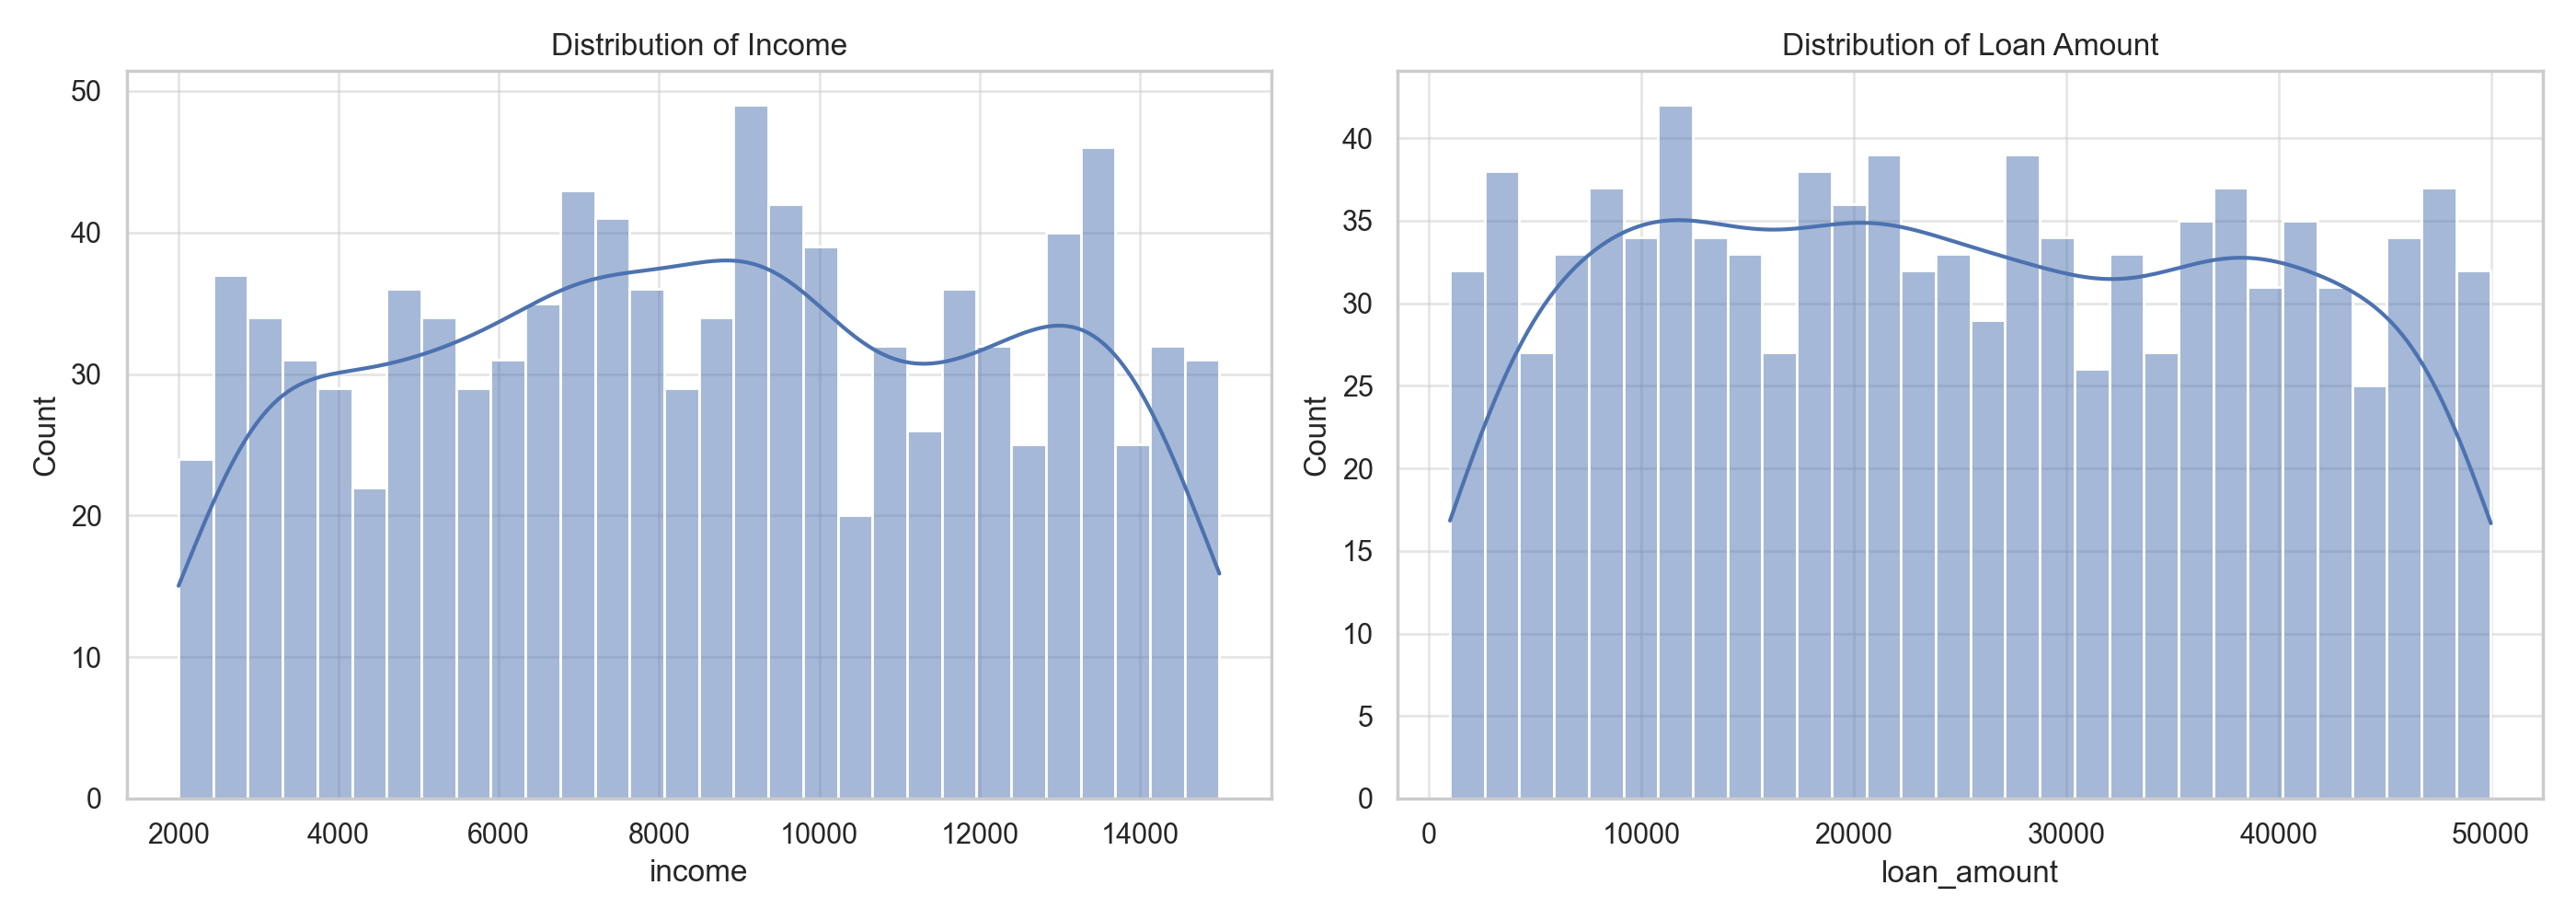
\includegraphics[width=\linewidth]{results/figures/eda_feature_distributions.png}
\end{minipage}
\hfill
\begin{minipage}{0.48\textwidth}
    \centering
    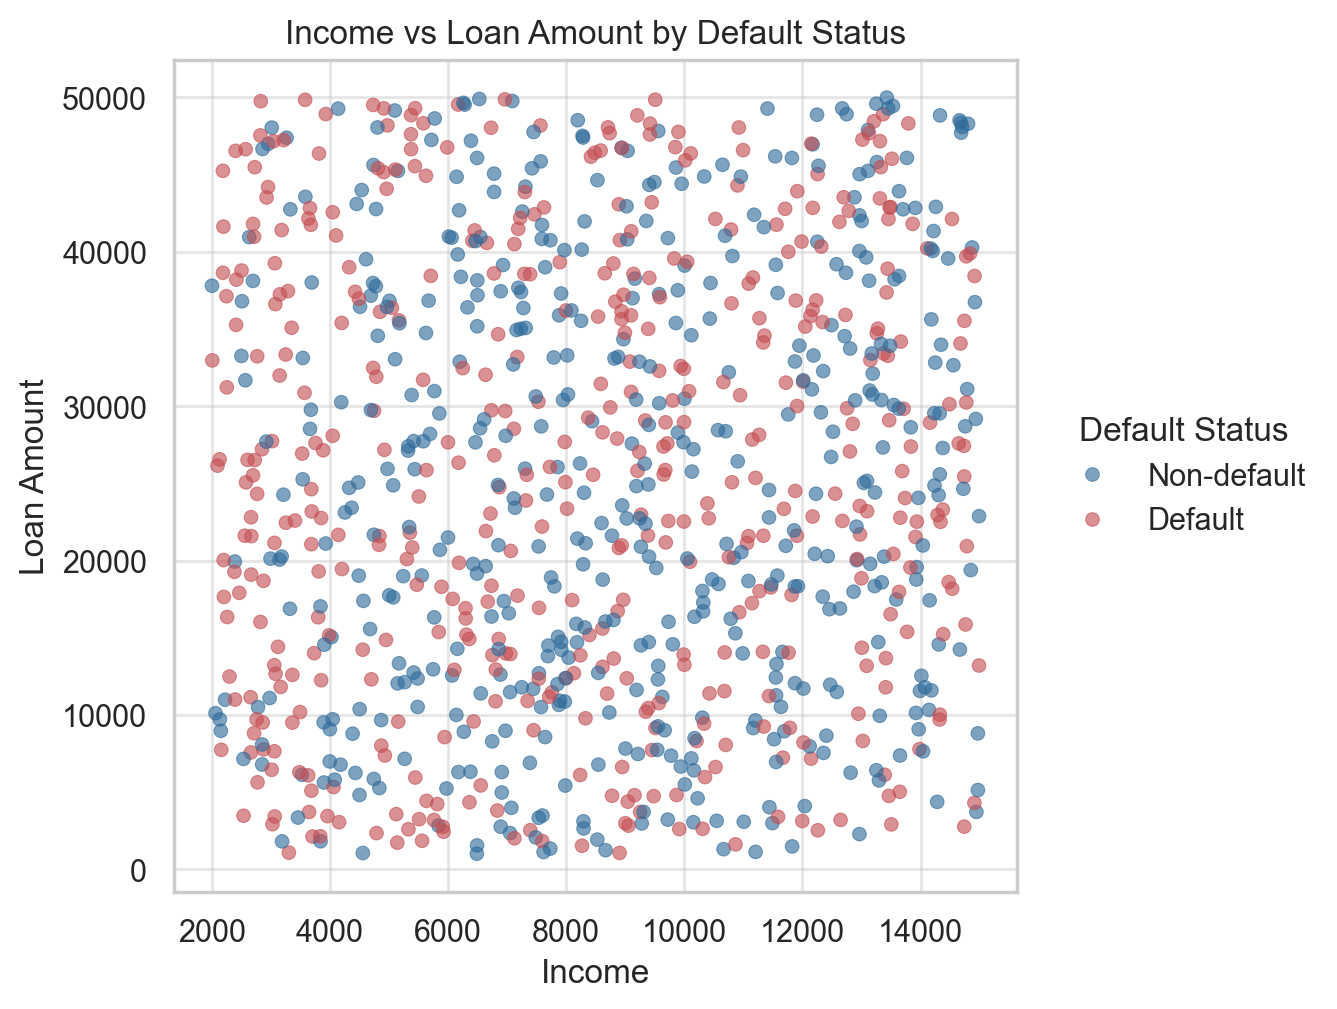
\includegraphics[width=\linewidth]{results/figures/eda_income_loan_scatter.png}
\end{minipage}
\caption{EDA distributions and the joint \texttt{income}--\texttt{loan\_amount} feature space.}
\end{figure}

\begin{figure}[H]
\centering
\begin{minipage}{0.48\textwidth}
    \centering
    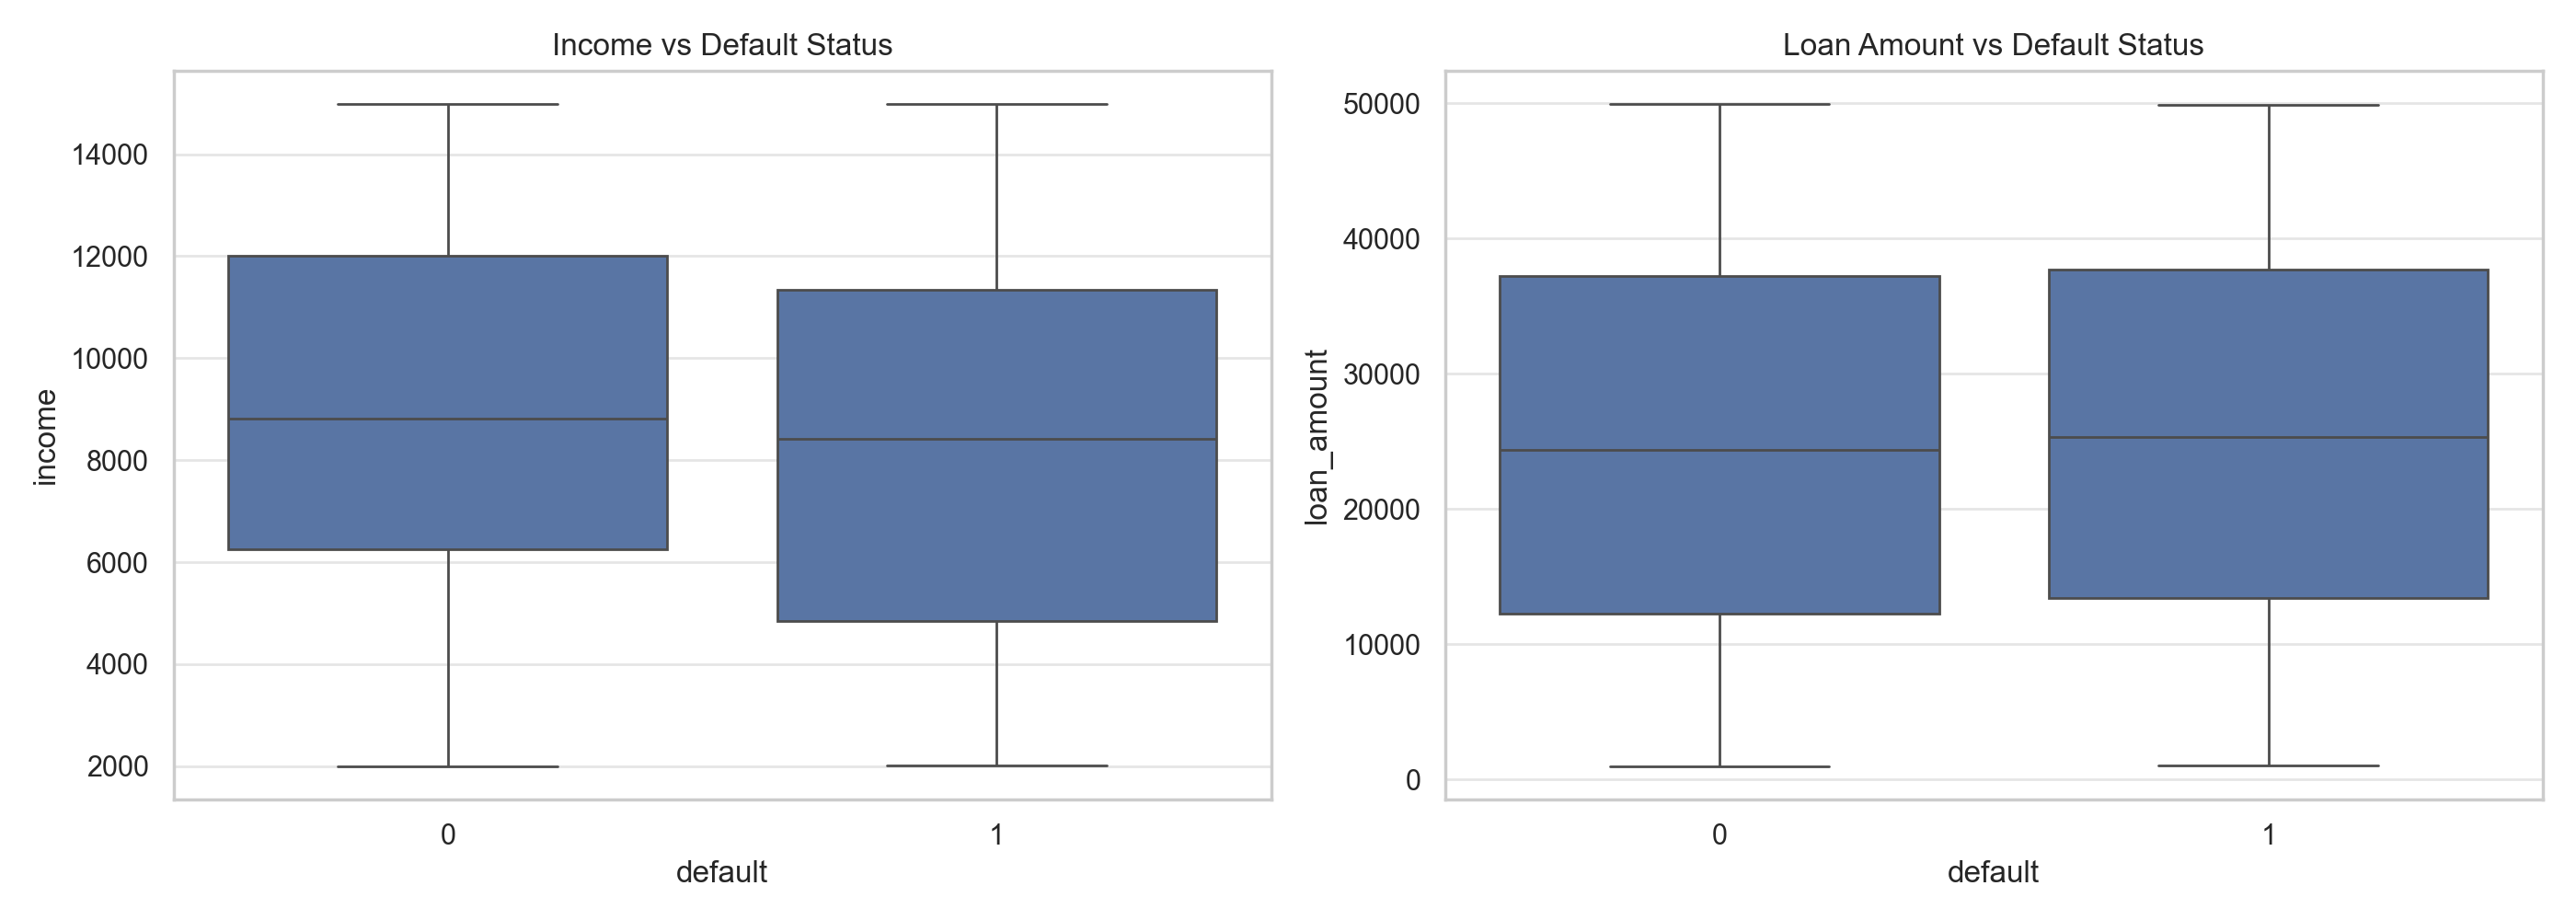
\includegraphics[width=\linewidth]{results/figures/eda_default_relationships.png}
\end{minipage}
\hfill
\begin{minipage}{0.40\textwidth}
    \centering
    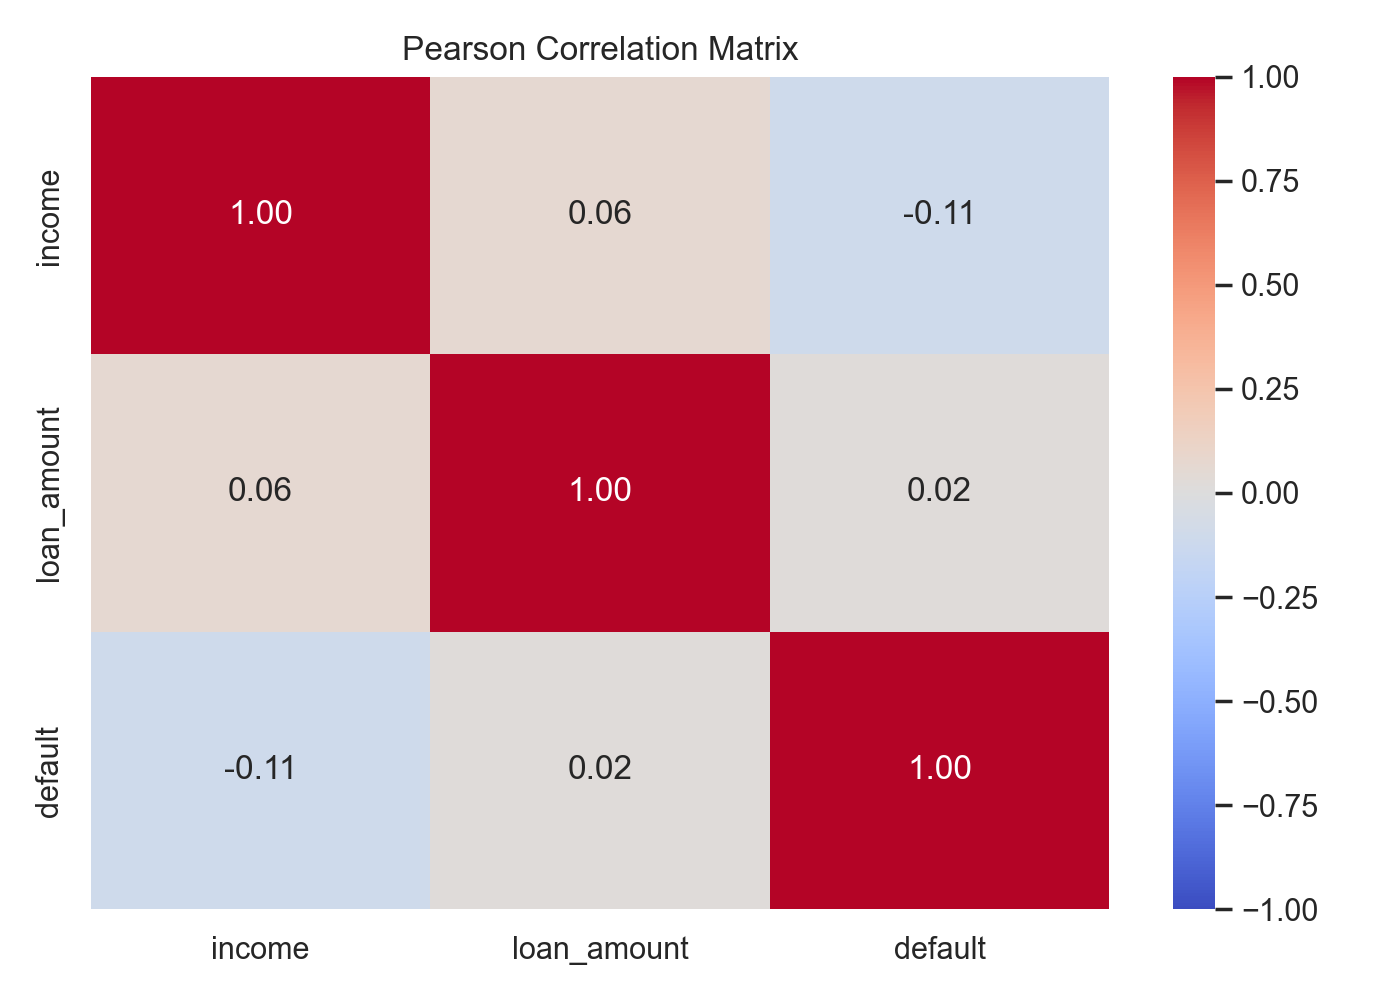
\includegraphics[width=\linewidth]{results/figures/eda_correlation_heatmap.png}
\end{minipage}
\caption{EDA comparisons by default status and the Pearson correlation matrix.}
\end{figure}

The numeric correlations are weak. Income has a small negative correlation with default ($-0.106$), while loan amount has a very small positive correlation with default ($0.021$). These values suggest that no single continuous predictor linearly separates the classes. The correlation between income and loan amount is also weak ($0.063$), so the two variables provide different information.

Outliers were checked using the interquartile range rule. For each continuous feature, an observation was treated as an outlier candidate if it fell below $Q_1-1.5\,IQR$ or above $Q_3+1.5\,IQR$. No outliers were detected for either continuous feature, so no winsorization or trimming was applied.

\subsubsection{Employment Status Pattern}

\textbf{Employment status shows a much stronger relationship with the target} than the continuous variables. Among employed applicants, the observed default rate is $0.257$. Among unemployed applicants, the observed default rate is $0.704$. This large difference motivates treating employment status as an important explanatory feature in the Logistic Regression baseline.

\begin{table}[htbp]
\centering
\caption{Observed default rate by employment status.}
\begin{tabular}{lrr}
\toprule
Employment Status & Count & Default Rate \\
\midrule
Employed & 486 & 0.257 \\
Unemployed & 514 & \best{0.704} \\
\bottomrule
\end{tabular}
\end{table}

\subsubsection{Feature Selection and Preprocessing Logic}

The final feature set contains three model inputs after preprocessing: standardized \texttt{income}, standardized \texttt{loan\_amount}, and the one-hot indicator \texttt{employment\_status\_Unemployed}. The column \texttt{loan\_id} is excluded because it is a unique identifier and would encourage memorization rather than generalization. The target column \texttt{default} is separated from the predictors.

\texttt{employment\_status} is encoded with one-hot encoding and \texttt{drop\_first=True}. Since there are two categories, this produces one indicator variable. The binary category is converted into a numerical indicator so the model can use category membership without imposing an artificial ordering. The dropped category is the employed baseline group, so the coefficient of \texttt{employment\_status\_Unemployed} measures the change relative to employed applicants.

\texttt{income} and \texttt{loan\_amount} are standardized using the training set mean and standard deviation:
\[
    z = \frac{x-\mu_{\text{train}}}{s_{\text{train}}}.
\]
The scaler is fit only on the training set and then applied to validation and test data. This prevents data leakage, because validation and test statistics are not used to transform the training data.

In the code, this transformation is implemented with \texttt{sklearn.preprocessing.StandardScaler}. Mathematically, \texttt{StandardScaler} estimates $\mu_{\text{train}}$ and $s_{\text{train}}$ from the training data and applies the same affine transformation to every later dataset. This makes each continuous feature dimensionless and comparable in scale, which is especially important for distance-based methods such as kNN.

\subsubsection{Train/Validation/Test Split}

The split strategy is 70\% training, 15\% validation, and 15\% test, with stratification on the target variable. This produces 700 training observations, 150 validation observations, and 150 test observations, each with three processed features. The training set fits model parameters, the validation set selects hyperparameters, and the test set is held out for final comparison.

The split is implemented with \texttt{sklearn.model\_selection.train\_test\_split}. This function randomly partitions the rows while the \texttt{stratify} argument preserves the class proportion of \texttt{default} in each subset. The fixed \texttt{random\_state} makes the split reproducible, so the reported metrics can be regenerated from the same data partition.

\subsection{1(b) Logistic Regression Baseline}

\subsubsection{Methodology}

Logistic Regression models the conditional probability that applicant $i$ defaults:
\[
    \hat{p}_i=P(y_i=1|\mathbf{x}_i)
    =
    \sigma(\mathbf{w}^{T}\mathbf{x}_i+b)
    =
    \frac{1}{1+\exp[-(\mathbf{w}^{T}\mathbf{x}_i+b)]}.
\]
The predicted class is 1 when $\hat{p}_i \geq 0.5$ and 0 otherwise.

The model is trained by minimizing binary cross-entropy:
\[
    \mathcal{L}(\mathbf{w},b)
    =
    -\frac{1}{n}\sum_{i=1}^{n}
    \left[
    y_i\log(\hat{p}_i)+(1-y_i)\log(1-\hat{p}_i)
    \right].
\]
This loss is appropriate for binary classification because it penalizes confident wrong probability estimates more strongly than uncertain wrong estimates.

The implementation uses \texttt{sklearn.linear\_model.LogisticRegression} with \texttt{max\_iter=1000}, \texttt{random\_state=42}, and the default L2 penalty with $C=1$. This estimator fits the weight vector and intercept by numerically optimizing the Logistic Regression objective, which is the binary cross-entropy loss above plus the default L2 penalty term. The optimization is iterative, so \texttt{max\_iter=1000} gives the solver enough steps to converge, while the fixed random seed improves reproducibility. Since the baseline is intended as a fixed reference classifier, its regularization strength is not tuned until the later explicit L1/L2 regularization study.

\subsubsection{Results}

\begin{table}[htbp]
\centering
\caption{Logistic Regression performance.}
\begin{tabular}{lrrr}
\toprule
Metric & Train & Validation & Test \\
\midrule
Accuracy $\uparrow$ & 0.720 & 0.700 & \best{0.760} \\
Precision $\uparrow$ & 0.703 & 0.675 & \best{0.740} \\
Recall $\uparrow$ & 0.736 & 0.740 & \best{0.781} \\
$F_1$-score $\uparrow$ & 0.719 & 0.706 & \best{0.760} \\
\bottomrule
\end{tabular}
\end{table}

\begin{table}[htbp]
\centering
\caption{Logistic Regression test-set confusion matrix.}
\begin{tabular}{lrr}
\toprule
 & Predicted 0 & Predicted 1 \\
\midrule
Actual 0 & \best{57} & 20 \\
Actual 1 & 16 & \best{57} \\
\bottomrule
\end{tabular}
\end{table}

The baseline achieves a test accuracy of 0.760 and a test $F_1$-score of 0.760. It correctly identifies 57 of 73 actual default cases and misses 16 defaults. It also incorrectly classifies 20 non-default cases as defaults. The balanced precision and recall indicate that the baseline is not simply predicting one class more aggressively than the other.

\subsection{1(c) Feature Interpretation Through Log-Odds}

For Logistic Regression, the log-odds are linear:
\[
    \log\left(\frac{\hat{p}_i}{1-\hat{p}_i}\right)
    =
    \mathbf{w}^{T}\mathbf{x}_i+b.
\]
Holding all other features fixed, a one-unit increase in feature $x_j$ changes the log-odds by $w_j$. The odds multiplier is $\exp(w_j)$.

For readability, the table label ``Unemployed indicator'' refers to \texttt{employment\_status\_Unemployed}.

\begin{table}[htbp]
\centering
\caption{Logistic Regression coefficients and odds ratios.}
\begin{tabular}{lrr}
\toprule
Feature & Coefficient & Odds Ratio \\
\midrule
Unemployed indicator & \best{1.907} & \best{6.731} \\
\texttt{income} & -0.311 & 0.733 \\
\texttt{loan\_amount} & 0.112 & 1.118 \\
\bottomrule
\end{tabular}
\end{table}

The unemployment coefficient is 1.907. Therefore, changing from the employed baseline group to the unemployed group increases the predicted default log-odds by 1.907, holding standardized income and standardized loan amount fixed. The odds ratio is $\exp(1.907)=6.731$, meaning the model estimates that unemployed applicants have about 6.7 times the odds of default compared with employed applicants with the same income and loan amount values.

The coefficient for income is negative, so higher income is associated with lower default risk after standardization. The loan amount coefficient is positive but much smaller, indicating a modest increase in default odds for larger loan amounts. Overall, the baseline confirms the EDA finding that employment status is the dominant feature in this dataset.

\section{Local Geometry and k-Nearest Neighbors Classification}

\subsection{2(a) Distance Metric and Feature Scaling}

\subsubsection{Methodology}

k-Nearest Neighbors is a non-parametric classifier. It does not estimate a global coefficient vector. Instead, for a test observation $\mathbf{x}$, it finds the $k$ closest training observations and predicts the class by majority vote.

The distance metric used in this project is Euclidean distance:
\[
    d(\mathbf{x}_i,\mathbf{x}_j)
    =
    \sqrt{\sum_{m=1}^{p}(x_{im}-x_{jm})^2}.
\]
Because this formula sums squared coordinate differences, variables with larger numerical ranges can dominate the distance. This is why standardization is essential for \texttt{income} and \texttt{loan\_amount}. Without scaling, the neighborhood structure may be determined mostly by the feature with the largest raw units rather than by the most predictive feature.

The implementation uses \texttt{sklearn.neighbors.KNeighborsClassifier}. For each validation or test point, this class computes distances from that point to the stored training observations in the processed feature space; with the default Minkowski metric and $p=2$, this is exactly Euclidean distance. It then selects the $k$ nearest training labels and predicts the class by majority vote. The default uniform voting rule is used, so each of the $k$ neighbors receives equal weight. The key hyperparameter is $k$, tuned in the next subsection.

\subsubsection{Scaling Sensitivity Results}

To directly test scaling sensitivity, the best selected kNN setting was evaluated on both standardized and unstandardized data.

\begin{table}[htbp]
\centering
\caption{kNN scaling sensitivity on the test set.}
\begin{tabular}{lrrrr}
\toprule
Input Data & Accuracy $\uparrow$ & Precision $\uparrow$ & Recall $\uparrow$ & $F_1$-score $\uparrow$ \\
\midrule
Unscaled & 0.560 & 0.564 & 0.425 & 0.484 \\
Scaled & \best{0.780} & \best{0.750} & \best{0.822} & \best{0.784} \\
\bottomrule
\end{tabular}
\end{table}

\textbf{The difference is large.} With unscaled inputs, test $F_1$-score is only 0.484. After standardization, test $F_1$-score rises to 0.784. This confirms that kNN is highly sensitive to feature scale and that the preprocessing step is not just cosmetic; it changes the actual neighborhood structure used for classification.

\subsection{2(b) Hyperparameter Tuning for $k$}

\subsubsection{Training Procedure}

The candidate values for $k$ are the odd integers from 1 to 51. Odd values reduce the chance of ties in binary classification. For each value of $k$, the model is fit on the training set and evaluated on the validation set. The validation $F_1$-score is the primary selection criterion because $F_1$ balances precision and recall for the default class.

\begin{figure}[htbp]
\centering
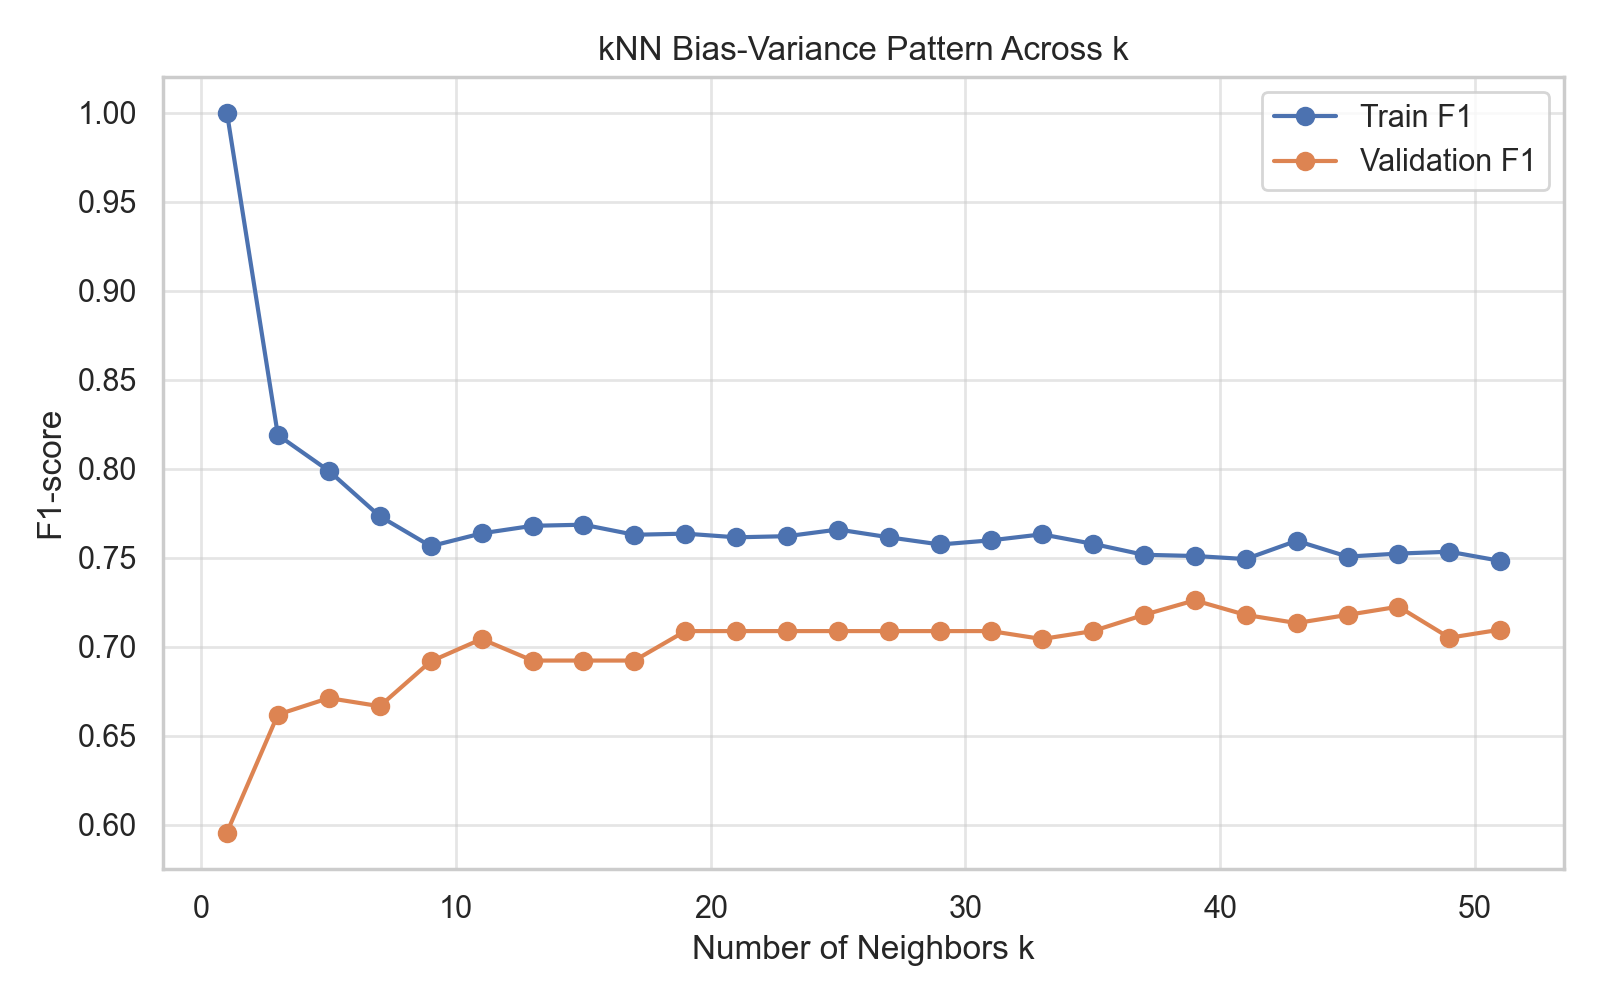
\includegraphics[width=0.72\textwidth]{results/figures/knn_train_validation_f1_by_k.png}
\caption{kNN train and validation $F_1$-score by $k$.}
\end{figure}

\subsubsection{Tuning Results and Bias--Variance Interpretation}

\begin{table}[htbp]
\centering
\caption{Representative kNN validation results.}
\begin{tabular}{rrrr}
\toprule
$k$ & Train $F_1$ $\uparrow$ & Validation Accuracy $\uparrow$ & Validation $F_1$ $\uparrow$ \\
\midrule
1 & \best{1.000} & 0.620 & 0.596 \\
3 & 0.819 & 0.680 & 0.662 \\
9 & 0.757 & 0.673 & 0.692 \\
39 & 0.751 & \best{0.713} & \best{0.726} \\
47 & 0.752 & \best{0.713} & 0.723 \\
51 & 0.748 & 0.700 & 0.710 \\
\bottomrule
\end{tabular}
\end{table}

At $k=1$, the training $F_1$-score is 1.000 because each training point is its own nearest neighbor. However, validation $F_1$-score is only 0.596. This is a classic high-variance pattern: the model fits local noise in the training set but generalizes poorly.

The \textbf{best selected value is $k=39$}, with validation accuracy 0.713 and validation $F_1$-score 0.726. Larger $k$ values smooth the decision boundary and reduce variance, but very large neighborhoods can increase bias because the classifier averages over too many points. The selected value therefore reflects a compromise between noisy local behavior and oversmoothing.

\subsection{2(c) Comparison with Logistic Regression}

\begin{table}[htbp]
\centering
\caption{kNN test-set confusion matrix for $k=39$.}
\begin{tabular}{lrr}
\toprule
 & Predicted 0 & Predicted 1 \\
\midrule
Actual 0 & \best{57} & 20 \\
Actual 1 & 13 & \best{60} \\
\bottomrule
\end{tabular}
\end{table}

\begin{table}[htbp]
\centering
\caption{Logistic Regression versus best kNN on the test set.}
\begin{tabular}{lrrrr}
\toprule
Model & Accuracy $\uparrow$ & Precision $\uparrow$ & Recall $\uparrow$ & $F_1$-score $\uparrow$ \\
\midrule
Logistic Regression & 0.760 & 0.740 & 0.781 & 0.760 \\
kNN ($k=39$) & \best{0.780} & \best{0.750} & \best{0.822} & \best{0.784} \\
\bottomrule
\end{tabular}
\end{table}

kNN improves test accuracy from 0.760 to 0.780 and $F_1$-score from 0.760 to 0.784. The improvement comes mainly from recall: kNN misses 13 actual defaults, while Logistic Regression misses 16. Both models make 20 false positive default predictions. This suggests that local neighborhoods help identify a few additional default cases without increasing false positives.

However, the improvement is modest. Logistic Regression remains competitive even though it is simpler and more interpretable. kNN also has limitations: it depends strongly on feature scaling, does not provide coefficients, and can become computationally expensive for larger datasets because predictions require distance calculations to training points.

\section{Polynomial Feature Expansion and Regularized Logistic Classification}

\subsection{3(a) Polynomial Feature Expansion}

\subsubsection{Methodology}

The goal of polynomial expansion is to allow a linear classifier to represent nonlinear relationships in the original feature space. The original processed feature set contains three variables: \texttt{employment\_status\_Unemployed}, standardized \texttt{income}, and standardized \texttt{loan\_amount}.

Polynomial expansion is applied to \texttt{income} and \texttt{loan\_amount} with degree 2 and \texttt{include\_bias=False}. In the code, this mapping is implemented with \texttt{sklearn.preprocessing.PolynomialFeatures}. Mathematically, \texttt{PolynomialFeatures} constructs a new design matrix by adding powers and interaction products of the selected input variables up to the specified degree. The employment-status indicator is kept as a separate linear feature. The expanded feature set is:
\[
    \{
    \texttt{employment\_status\_Unemployed},
    \texttt{income},
    \texttt{loan\_amount},
    \texttt{income}^2,
    \texttt{income}\cdot\texttt{loan\_amount},
    \texttt{loan\_amount}^2
    \}.
\]

\begin{table}[htbp]
\centering
\caption{Polynomial feature expansion summary.}
\begin{tabular}{ll}
\toprule
Quantity & Value \\
\midrule
Original feature count & 3 \\
Expanded feature count & 6 \\
Polynomial degree & 2 \\
Expanded continuous terms & $\texttt{income}^2$, $\texttt{income}\times\texttt{loan\_amount}$, $\texttt{loan\_amount}^2$ \\
\bottomrule
\end{tabular}
\end{table}

A Logistic Regression model is still linear in the expanded feature matrix, but it becomes nonlinear in the original \texttt{income}--\texttt{loan\_amount} plane. This helps the model represent curved or interaction-based decision boundaries while preserving the basic probability model.

Although the response is binary and the final classifier is Logistic Regression, the polynomial component follows the same course idea as Polynomial Regression: expanding input variables into powers and interactions so that a linear model in the expanded space can represent nonlinear structure in the original feature space.

\subsection{3(b) L2 and L1 Regularized Logistic Regression}

\subsubsection{Mathematical Formulation}

The unregularized binary cross-entropy loss is denoted by $\mathcal{L}(\mathbf{w},b)$. L2-regularized Logistic Regression minimizes
\[
    \mathcal{J}_{L2}(\mathbf{w},b)
    =
    \mathcal{L}(\mathbf{w},b)
    +
    \lambda\sum_{j=1}^{p}w_j^2.
\]
The squared penalty discourages large coefficients and tends to shrink all coefficients smoothly.

L1-regularized Logistic Regression minimizes
\[
    \mathcal{J}_{L1}(\mathbf{w},b)
    =
    \mathcal{L}(\mathbf{w},b)
    +
    \lambda\sum_{j=1}^{p}|w_j|.
\]
The absolute-value penalty can set coefficients exactly to zero, making it useful for sparse feature selection.

In this classification setting, the same L2 and L1 penalty ideas used in Ridge and Lasso are added to the Logistic Regression loss rather than to the ordinary least-squares loss. Thus the penalty controls coefficient size and sparsity while the cross-entropy term still fits class probabilities.

In \texttt{scikit-learn}, the parameter $C$ is the inverse of regularization strength. Relative to the lecture notation above, larger $\lambda$ means a stronger penalty, while scikit-learn uses $C \propto 1/\lambda$; therefore smaller $C$ means stronger regularization and larger $C$ means weaker regularization. The tested grid is
\[
    C \in \{0.01,0.03,0.1,0.3,1,3,10,30,100\}.
\]
The implementation again uses \texttt{sklearn.linear\_model.LogisticRegression}, but now the \texttt{penalty} argument is set to either \texttt{l1} or \texttt{l2}. The \texttt{liblinear} solver is chosen because it supports both penalties in this binary-classification setting, so the same estimator class can implement the Ridge-style L2 objective and the Lasso-style L1 objective.

\subsubsection{Fixed $C=1$ Comparison}

As an initial comparison, L1 and L2 Logistic Regression are trained with $C=1$. Both fixed-regularization models achieve the same test accuracy (0.773) and $F_1$-score (0.776), so the more important comparison is how validation performance changes across the regularization grid.

\subsubsection{Regularization Tuning}

\begin{figure}[H]
\centering
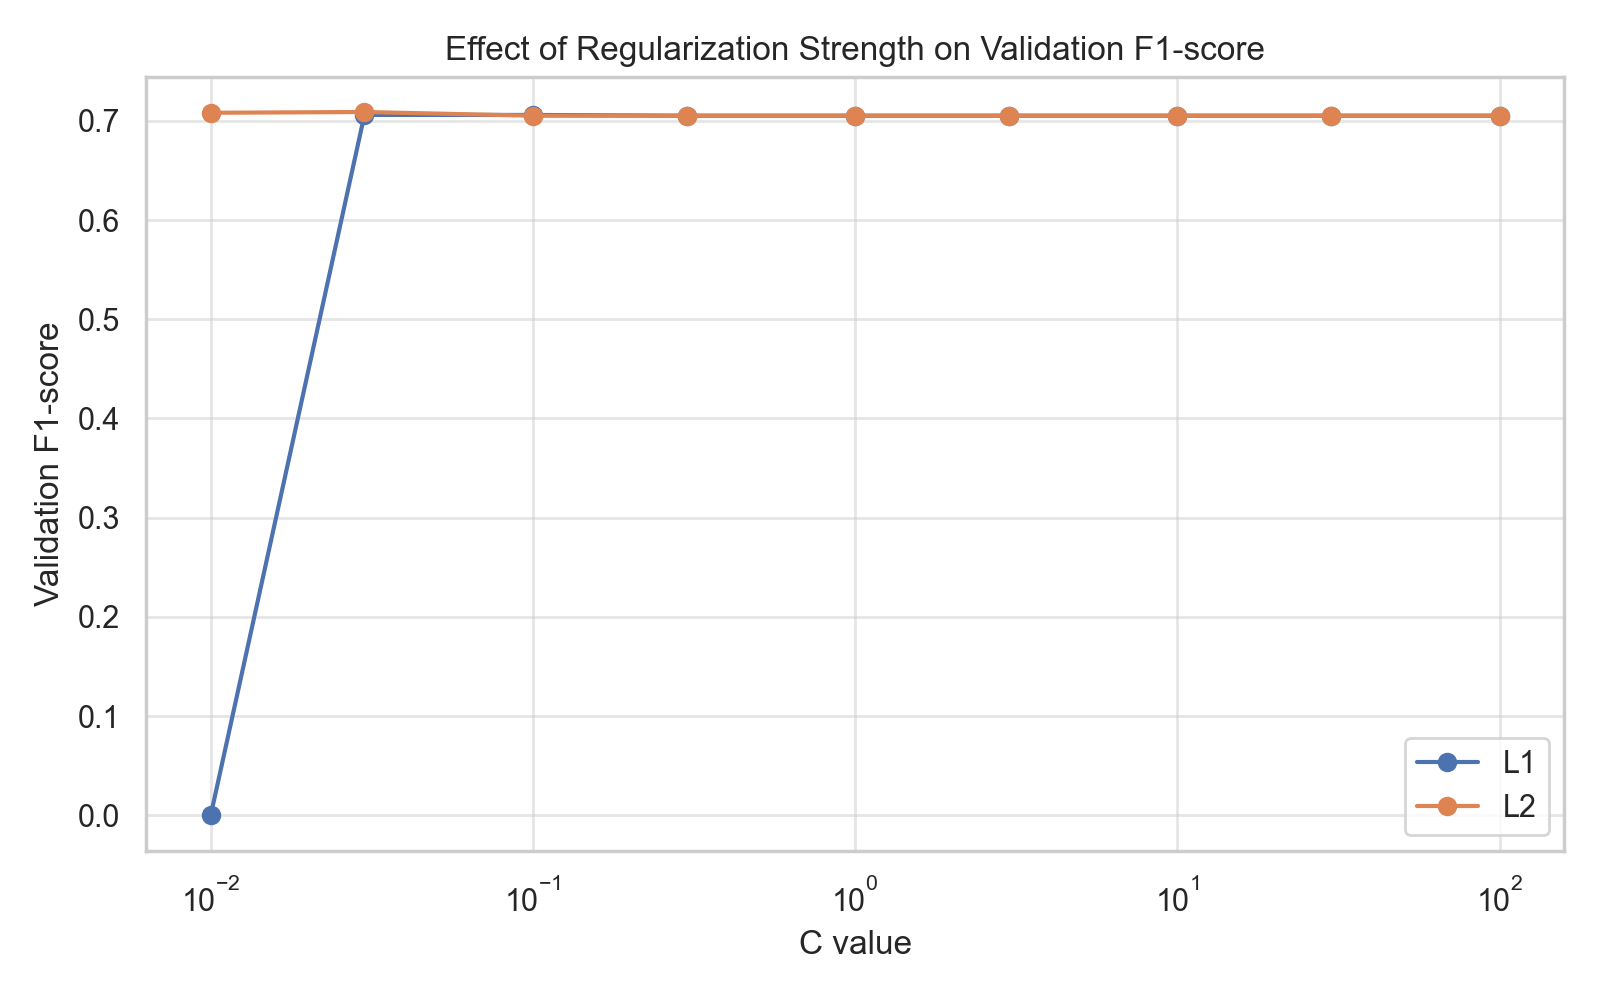
\includegraphics[width=0.74\textwidth]{results/figures/regularization_validation_f1_by_C.png}
\caption{Validation $F_1$-score across regularization strengths.}
\end{figure}

\vspace{-0.5em}

\begin{table}[H]
\centering
\caption{Representative regularization tuning results.}
\setlength{\tabcolsep}{7pt}
\begin{tabular}{lrrr}
\toprule
Penalty & $C$ & Validation Accuracy $\uparrow$ & Validation $F_1$ $\uparrow$ \\
\midrule
L2 & 0.01 & 0.687 & 0.708 \\
L1 & 0.01 & 0.513 & 0.000 \\
L2 & 0.03 & 0.693 & \best{0.709} \\
L1 & 0.03 & \best{0.700} & 0.706 \\
L2 & 1.00 & 0.693 & 0.705 \\
L1 & 1.00 & 0.693 & 0.705 \\
\bottomrule
\end{tabular}
\end{table}

\vspace{-0.5em}

The \textbf{best validation-selected regularized model}, by a very small margin, is the L2 polynomial Logistic Regression model with $C=0.03$. Its validation $F_1$-score is 0.709 and its test $F_1$-score is 0.800, the strongest observed test result. The validation score is not dramatically higher than the other regularized models, so the improvement should be interpreted cautiously.

\begin{table}[H]
\centering
\caption{Best polynomial Logistic Regression confusion matrix.}
\begin{tabular}{lrr}
\toprule
 & Predicted 0 & Predicted 1 \\
\midrule
Actual 0 & \best{57} & 20 \\
Actual 1 & 11 & \best{62} \\
\bottomrule
\end{tabular}
\end{table}

\subsection{3(c) Effect of Regularization on Feature Weights}

\subsubsection{Coefficient Comparison}

\begin{table}[H]
\centering
\caption{L1 and L2 polynomial coefficients at $C=1$.}
\begin{tabular}{lrr}
\toprule
Feature & L2 Coefficient & L1 Coefficient \\
\midrule
Unemployed indicator & \best{1.954} & \best{1.984} \\
\texttt{income} & -0.302 & -0.299 \\
\texttt{income}$^2$ & 0.276 & 0.275 \\
\texttt{income}$\times$\texttt{loan\_amount} & -0.140 & -0.135 \\
\texttt{loan\_amount} & 0.082 & 0.077 \\
\texttt{loan\_amount}$^2$ & 0.023 & 0.016 \\
\bottomrule
\end{tabular}
\end{table}

At $C=1$, the L1 and L2 coefficients are similar and neither model is strongly sparse. Employment status remains the dominant predictor. The income coefficient remains negative, while the income-squared term is positive. This suggests some curvature in the income relationship, although the effect size is much smaller than the employment-status effect.

\subsubsection{L1 Sparsity}

\begin{figure}[H]
\centering
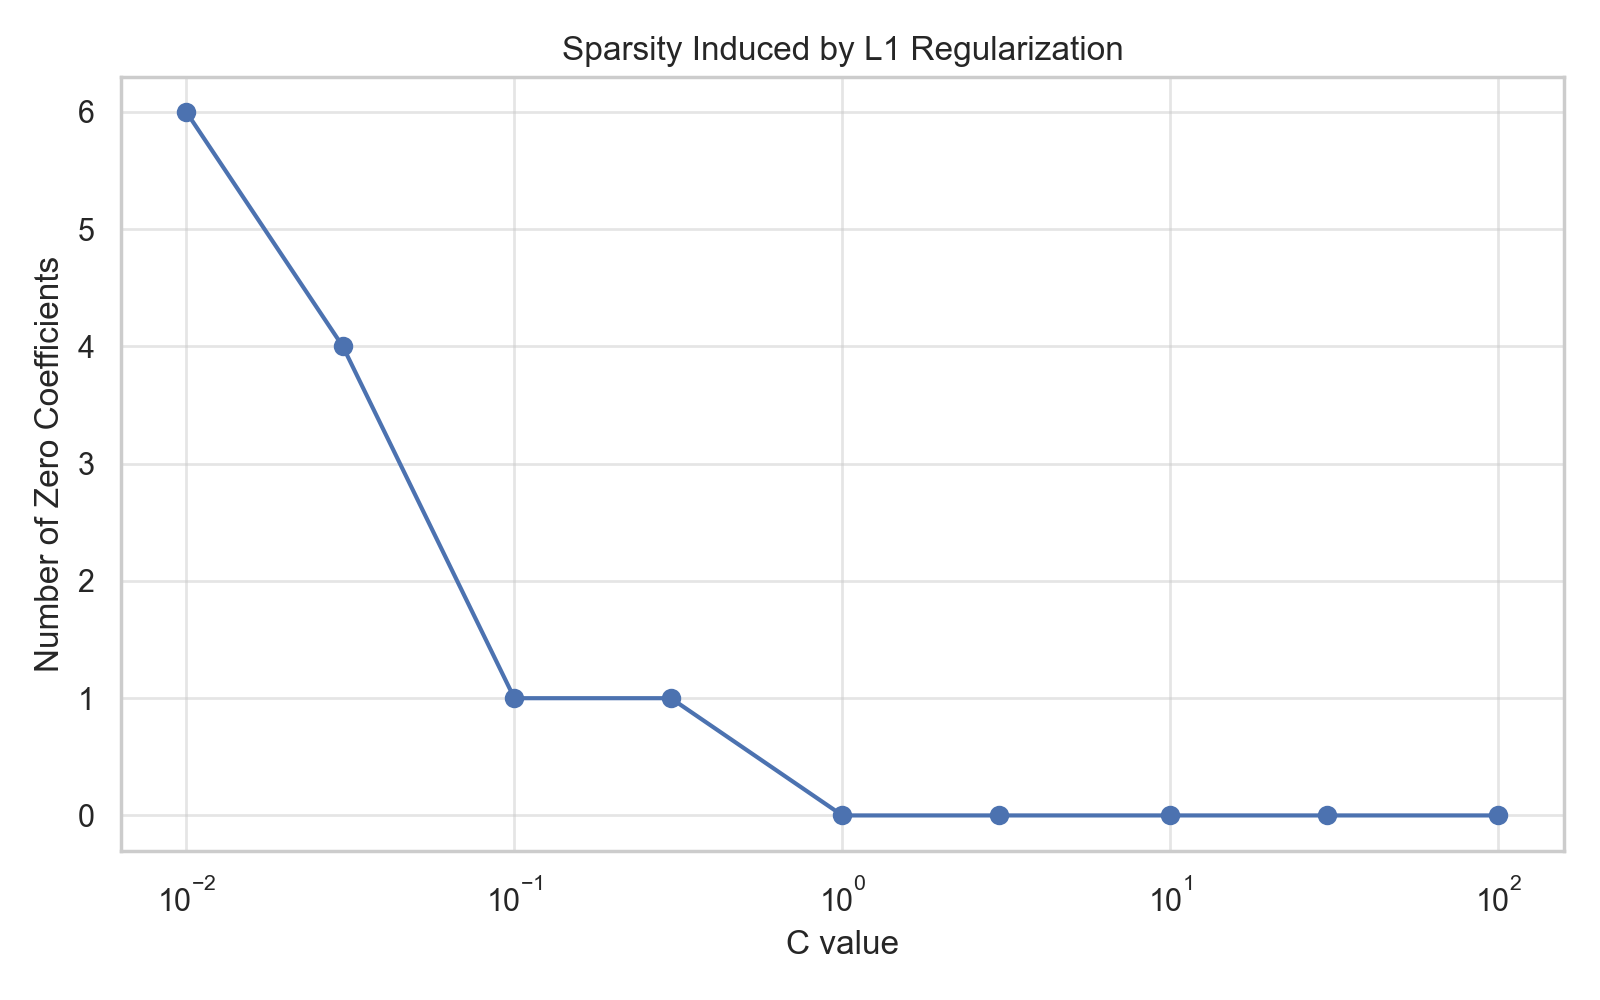
\includegraphics[width=0.62\textwidth]{results/figures/l1_sparsity_by_C.png}
\caption{L1 sparsity across regularization strengths.}
\end{figure}

L1 regularization produces sparsity when the regularization is strong. At $C=0.01$, all six coefficients are set to zero and validation $F_1$-score collapses to 0.000, which indicates underfitting. At $C=0.03$, four coefficients are zero: \texttt{loan\_amount}, \texttt{income} squared, the income--loan amount interaction, and \texttt{loan\_amount} squared. For $C=1$ and larger, no coefficients are zero.

This pattern shows both the value and the risk of L1 regularization. It can identify unnecessary terms and simplify the model, but excessive regularization can remove too much information and destroy predictive performance. L2 regularization is more stable in this project because it shrinks coefficients without eliminating them completely.

\section{Final Model Comparison and Analysis}

\subsection{Overall Test Performance}

\begin{table}[htbp]
\centering
\caption{Final model comparison on the test set.}
\begin{tabular}{lrrrr}
\toprule
Model & Accuracy $\uparrow$ & Precision $\uparrow$ & Recall $\uparrow$ & $F_1$-score $\uparrow$ \\
\midrule
Poly Logistic (L2, selected $C=0.03$) & \best{0.793} & \best{0.756} & \best{0.849} & \best{0.800} \\
kNN ($k=39$) & 0.780 & 0.750 & 0.822 & 0.784 \\
Poly Logistic (L2, fixed $C=1$) & 0.773 & 0.747 & 0.808 & 0.776 \\
Poly Logistic (L1, fixed $C=1$) & 0.773 & 0.747 & 0.808 & 0.776 \\
Logistic Regression & 0.760 & 0.740 & 0.781 & 0.760 \\
\bottomrule
\end{tabular}
\end{table}

The \textbf{best test $F_1$-score is achieved by the validation-selected polynomial Logistic Regression model} with L2 regularization and $C=0.03$. Its test $F_1$-score is 0.800. The next best model is kNN with $k=39$, with test $F_1$-score 0.784. The baseline Logistic Regression model has test $F_1$-score 0.760.

The ranking suggests that additional flexibility helps, but the improvement is moderate. The best polynomial model improves $F_1$-score by 0.040 over the baseline and by 0.016 over kNN. This is meaningful but not large enough to claim that one method is universally superior. The result is better interpreted as evidence that mild nonlinear expansion and regularization can improve this particular split of this synthetic dataset.

\subsection{Confidence Intervals and Statistical Caution}

Because the test set contains only 150 observations, small differences in accuracy may not be statistically decisive. A 95\% Wilson binomial confidence interval for test accuracy gives the following ranges:

\begin{table}[htbp]
\centering
\caption{Approximate 95\% Wilson confidence intervals for test accuracy.}
\begin{tabular}{lcc}
\toprule
Model & Test Accuracy $\uparrow$ & 95\% CI \\
\midrule
Poly Logistic (L2, selected $C=0.03$) & \best{0.793} & [0.722, 0.850] \\
kNN ($k=39$) & 0.780 & [0.707, 0.839] \\
Poly Logistic (L2, fixed $C=1$) & 0.773 & [0.700, 0.833] \\
Poly Logistic (L1, fixed $C=1$) & 0.773 & [0.700, 0.833] \\
Logistic Regression & 0.760 & [0.686, 0.821] \\
\bottomrule
\end{tabular}
\end{table}

The intervals overlap substantially. Therefore, the safest conclusion is not that the polynomial model is conclusively better in a statistical sense, but that it achieved the best observed test performance under the chosen split. These intervals are computed for test accuracy because accuracy is a binomial proportion over correct and incorrect predictions. Since $F_1$-score is a nonlinear function of precision and recall, uncertainty for $F_1$ would be better estimated using bootstrap resampling or repeated stratified splits.

\subsection{Strengths of the Approach}

The preprocessing pipeline worked well because it separated training, validation, and test information cleanly. Standardization was fit only on the training set, preventing data leakage. Stratification preserved the target distribution across splits. These choices make the model comparison more reliable.

Logistic Regression worked well as an interpretable baseline. It achieved respectable performance and provided direct coefficient interpretation. The unemployment coefficient was large and positive, matching the EDA default-rate difference between employed and unemployed applicants.

kNN worked well after scaling. The scaled-versus-unscaled comparison demonstrated exactly why preprocessing matters for distance-based methods. kNN improved recall relative to the baseline, suggesting that local neighborhood structure captures some default cases that the linear baseline misses.

Polynomial expansion with L2 regularization produced the strongest test $F_1$-score. This suggests that nonlinear terms involving income and loan amount add some useful information, even though employment status remains the dominant feature.

\subsection{Weaknesses and Failure Cases}

Unscaled kNN performed poorly. Its test $F_1$-score was 0.484, which confirms that raw feature scales distort Euclidean distance. This failure is useful because it supports the methodological claim that feature scaling is essential for distance-based classifiers.

Very small kNN neighborhoods also did not generalize well. At $k=1$, the training $F_1$-score was perfect, but validation $F_1$-score was only 0.596. This is a clear overfitting pattern.

Strong L1 regularization also failed when $C$ was too small. At $C=0.01$, all coefficients were zero and validation $F_1$-score was 0.000. This shows that sparsity is beneficial only when the penalty is not so strong that the model discards all predictive information.

\subsection{Limitations and Future Directions}

The main limitation is dataset size and feature scope. The dataset has only 1000 observations and three predictive inputs after preprocessing. Real credit-risk models typically use many additional variables, such as credit history, debt-to-income ratio, loan term, interest rate, payment history, and macroeconomic context. Because this dataset is synthetic, the results should be interpreted as a modeling exercise rather than a deployable underwriting system.

Another limitation is that the final comparison uses one train/validation/test split. Although the split is stratified and reproducible, performance estimates can vary across random splits. Future work should use repeated stratified cross-validation to estimate performance variability more robustly.

The current project uses a default classification threshold of 0.5 for Logistic Regression. In real credit-risk applications, the decision threshold should be tuned based on the relative costs of false positives and false negatives. Future work could study precision--recall curves, ROC curves, threshold optimization, and cost-sensitive classification.

Finally, the project compares a limited set of course-approved methods. Future work within the same course scope could add PCA-based preprocessing, k-means exploratory grouping, and repeated stratified cross-validation. More advanced models are intentionally excluded because the assignment restricts the project to methods covered in class.

\section{Conclusion}

The complete analysis shows that the loan default task benefits from comparing models with different assumptions. Logistic Regression provides an interpretable baseline and shows that unemployment strongly increases estimated default risk. kNN demonstrates the importance of local geometry and feature scaling. \textbf{Polynomial Logistic Regression with L2 regularization achieves the best observed test $F_1$-score}, suggesting that mild nonlinear feature expansion helps in this dataset.

At the same time, the performance differences are moderate and the confidence intervals overlap. The most defensible conclusion is that \textbf{regularized nonlinear expansion and scaled local classification can improve performance over a simple baseline}, but the gains should be interpreted with caution due to the limited test size and synthetic nature of the dataset.

\begin{thebibliography}{9}
\bibitem{seker_kaggle}
Şahide Şeker. \textit{Loan Default Prediction Dataset}. Kaggle. Available at:
\url{https://www.kaggle.com/datasets/sahideseker/loan-default-prediction-dataset}.
Accessed May 4, 2026.

\bibitem{pandas_docs}
pandas development team. \textit{pandas documentation}. Available at:
\url{https://pandas.pydata.org/docs/}.

\bibitem{sklearn_docs}
scikit-learn developers. \textit{scikit-learn: machine learning in Python}. Available at:
\url{https://scikit-learn.org/stable/}.

\bibitem{sklearn_paper}
Fabian Pedregosa et al. \textit{Scikit-learn: Machine Learning in Python}. Journal of Machine Learning Research, 12:2825--2830, 2011.

\bibitem{matplotlib_docs}
Matplotlib development team. \textit{Matplotlib documentation}. Available at:
\url{https://matplotlib.org/stable/}.

\bibitem{seaborn_docs}
seaborn development team. \textit{seaborn documentation}. Available at:
\url{https://seaborn.pydata.org/}.
\end{thebibliography}

\end{document}
